
We will formalize the amplitude and phase distance between functions of
$\mathcal{F}$, which will come in a natural way due to the properties of the
metric.

Firstly, before we proceed to define the phase and amplitude space, we will see
an analogy with the rotations on the complex plane, which will be very useful to
understand the role played by each of the magnitudes in our manifold.

Let  $z_1, z_2$ be two points in $\mathbb{C}$, as it is illustrated in the
figure \ref{FIG:ROTATION}, when it is applied a rotation on the plane, their
distance remains invariant, i.e., it is an action by isometries, as the
reparameterizations on our manifold.


\begin{figure}[Rotation in complex plane]{FIG:ROTATION}{Rotation in complex plane}

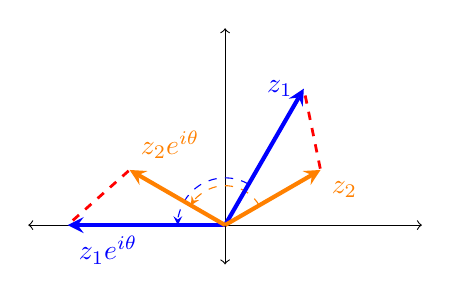
\begin{tikzpicture}
  %% Axis
  \draw[<->] (-2.5,0)--(2.5,0);%% node[above]{$\operatorname{Re}\{z\}$};
  \draw[<->] (0,-0.5)--(0,2.5);%% node[above]{$\operatorname{Im}\{z\}$};

  \draw[blue, -stealth, dashed](0.3, 0.5196) arc(60:180:0.6);
  \draw[orange, -stealth, dashed](0.433, 0.25) arc(30:150:0.5);

  %% Original vectors
  \draw[line width=1.5pt,blue,-stealth](0,0)--(1, 1.732) node[anchor=  east]{${z_1}$};
  \draw[line width=1.5pt,orange,-stealth](0,0)--(1.2124, 0.7) node[anchor= north west]{${z_2}$};
  \draw[line width=1pt,red, dashed, shorten <=2.5](1, 1.732)--(1.2124, 0.7);% node[anchor= south west]{${| z_1 - z_2| }$};

  %% Rotated vectors
  \draw[line width=1.5pt,blue,-stealth](0,0)--(-2, 0) node[anchor= north west]{${z_1 e^{i\theta}}$};
  \draw[line width=1.5pt,orange,-stealth](0,0)--(-1.2124, 0.7) node[anchor= south west]{${z_2 e^{i\theta}}$};
  \draw[line width=1pt,red, dashed, shorten <=2.5](-2, 0)--(-1.2124, 0.7);% node[anchor= south east]{${| z_1e^{i\theta} - z_2e^{i\theta}| }$};

\end{tikzpicture}
\end{figure}

The variability between two vectors in the plane can be completely specified by
the angle between them, which will play the role of the phase in our space, and
the difference of their modules, which will be equivalent to the distance
between the vector once aligned.

\begin{figure}[Phase and amplitude in the complex plane]{FIG:COMPLEX}{Phase and amplitude in the complex plane}

\subfigure[SBFIG:COMPLEX2]{Angle between vectors}{

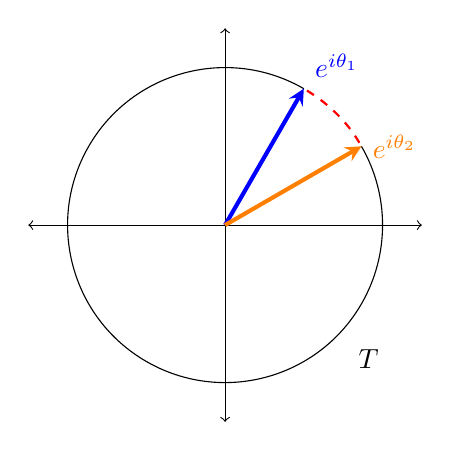
\begin{tikzpicture}

%% Axis
\draw[<->] (-2.5,0)--(2.5,0) ; %%node[right]{$\operatorname{Re}\{z\}$};
\draw[<->] (0,-2.5)--(0,2.5) ; %%node[above]{$\operatorname{Im}\{z\}$};

% Unit circle
 \draw(1, 1.732) arc(60:390:2);
 \draw[red, thick, dashed, shorten <=1.5] (1.732, 1) arc(30:60:2);
 \node[text width=0.2] at (1.7,-1.7) {$\mathbb{T}$};

%% Original vectors
\draw[line width=1.5pt,blue,-stealth](0,0)--(1, 1.732) node[anchor=  south west]{${e^{i \theta_1}}$};
\draw[line width=1.5pt,orange,-stealth](0,0)--(1.732, 1) node[anchor=  west]{${e^{i \theta_2}}$};



\end{tikzpicture}



} \quad

\subfigure[SBFIG:COMPLEX2]{Distance in $\mathb{C}/\mathbb{T}$}{

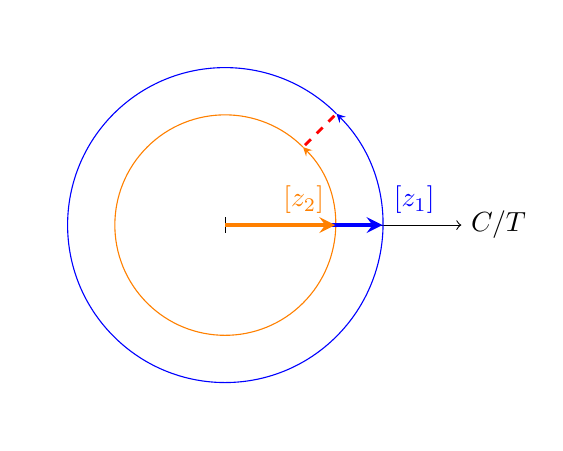
\begin{tikzpicture}

%% Fake axes to have the same margins
\draw[white, opacity=0] (-2.5,0)--(2.5,0) ; %%node[right]{$\operatorname{Re}\{z\}$};
\draw[white, opacity=0] (0,-2.5)--(0,2.5) ; %%node[above]{$\operatorname{Im}\{z\}$};

%% Axis
\draw[|->] (0,0)--(3,0) node[right]{$\mathbb{C}/\mathbb{T}$};


%%\draw[orange] (0, 0) circle (1.4);
%%\draw[blue] (0, 0) circle (2);

 \draw[orange, -stealth] (0.9899, 0.9899) arc(45:405:1.4);
 \draw[blue, -stealth] (1.4142, 1.4142) arc(45:405:2);

%% Rotated vectors
\draw[line width=1.5pt,blue,-stealth](0,0)--(2, 0) node[anchor= south west]{${[z_1]}$};
\draw[line width=1.5pt,orange,-stealth](0,0)--(1.4, 0) node[anchor= south east]{${[z_2]}$};
\draw[line width=1pt,red, dashed, shorten <=1](0.9899, 0.9899)--(1.4142, 1.4142);% node[anchor= south west]{$|[z_1] - [z_2]|$};




\end{tikzpicture}


}

\end{figure}


This distance of the vectors aligned may be understood as a distance in the
quotient space $\mathbb{C} / \mathbb{T}$, where $\mathbb{T}$ is the unit circle,
which it is isomorph to the group of rotations in the plane $SO(2)$. In this
quotient space we will define the equivalence classes
$[z] = \{z e^{i \theta} : \theta \in [0, 2\pi]\}$.

In the case of our manifold, let $q \in \mathbb{L}^2$ be a SRSF. We will define
its orbit under $\Gamma as [q] = \{(q, \gamma) : \gamma \in \Gamma \}$, in
other words, it is the set of reparameterizations associated to q. In the
figure \ref{ORBIT1} it is shown some reparameterizations associated  to a function
of $\mathscr{F}$ and their corresponding SRSF's in \ref{ORBIT2}.


\begin{figure}[Functions in the same orbit]{FIG:ORBIT}{Functions in the same orbit}
  \subfigure[SBFIG:ORBIT1]{$f \circ \gamma_i$}{\image{7cm}{}{0-empty}} \quad
  \subfigure[SBFIG:ORBIT2]{$(q,\gamma_i)$}{\image{7cm}{}{0-empty}}
\end{figure}

We will denote amplitude space $\mathscr{A}= \mathbb{L}^{2} / \Gamma$  to the
set of these orbit. In this space the phase variation is incorporated within
equivalence classes, while the amplitude variation appears across equivalence
classes, as in the analogy with the complex plane. We will endow the space with
the elastic metric, defined as

$$
d_{a}\left(\left[q_{1}\right],\left[q_{2}\right]\right)=\inf _{
\gamma_{1}, \gamma_{2} \in \tilde{\Gamma}}\left(\left\|\left(q_{1},
 \gamma_{1}\right)-\left(q_{2}, \gamma_{2}\right)\right\|\right),
$$

To quantify the other source of variability, we will define the phase space,
which will denoted as
$\Gamma = {\gamma :[0,1] \rightarrow[0,1]  : \gamma \, is \, a \, boundary-preserving \, diffeomorphism}$,
for which the natural distance will be given by the Fisher-Rao metric.

Let $\gamma \in \Gamma$ be a warping function, under the Fisher-Rao metric,
their norm will be 1, thus

$$
\| \gamma \|_\Gamma^2 = \| SRSF(\gamma)\|_L2^2 =  \| \dot \gamma\|_L2^2 =
\int_0^1 \sqrt{\dot \gamma (t)} \sqrt{\dot \gamma (t)}dt =
\int_0^1 \dot \gamma(t)dt = \gamma(1) - \gamma(0) = 1.
$$

The SRSF transform will be an isometry between $\Gamma$ and the unit sphere in
$\mathbb{L}^2$, also known as Hilbert Sphere
$\mathbb{S}_\infty = \{ \psi \in \mathbb{L}^2 : \|\psi\|_{\mathbb{L}^2}=1\}$.
To calculate distances in $\Gamma$ we will apply this transformation which will
allow us to use the structure of $\mathbb{S}_\infty$.

Let $\gamma_1, \gamma_2$ be in $\Gamma$ and $\psi_1=\sqrt{\dot \gamma_1},
\psi_2=\sqrt{\dot \gamma_1}$ be their SRSF, their distance in $\Gamma$ will be
given by

$$
d_{phase}(\gamma_1, \gamma_2) = d_{\psi}(\psi_1, \psi_2) =
cos^{-1}(\int_0^1 \psi_1(t) \psi_2(t) dt).
$$

This result is analogous to the rotations in the plane, where the cosine of
the angle between two unit vectors will be given by the inner product.
If we apply a rotation to two vectors, their angle remains invariant, in our
case the phase distance will be invariant to common reparameterizations due to
the properties of the Fisher-Rao metric.

Let $f_1, f_2$ be functions in $\mathcal{F}$, their relative phase is defined as

$$
\left(\gamma_{1}^{*}, \gamma_{2}^{*}\right)=\underset{\gamma_{1}, \gamma_{2} \in \Gamma}{\operatorname{argmin}}\left(\left\|\left(q_{1}, \gamma_{1}\right)-\left(q_{2}, \gamma_{2}\right)\right\|\right) \in \Gamma \times \Gamma.
$$

Which will allow us to calculate the phase variability between them,
as a generalization of the notion of an angle. The phase distance between these
functions will be the distance of their relative phase 
$d_{phase} (\gamma_{1}^{*}, \gamma_{2}^{*}\right)$.
